%!TEX root = main.tex


Human perception naturally reasons about information even if it is not fully visible~\cite{palmer1999vision}. The ability to reason about occlusions permits reaction based on the invisible. %anticipate and quickly react. 
For instance, when switching lanes on a highway, a partial view of a car and its movement through the rear-window is enough to understand the situation by completing the occluded parts subconsciously. This in turn helps to prevent collisions. 

%!TEX root = main.tex

\begin{figure*}[t]
\centering
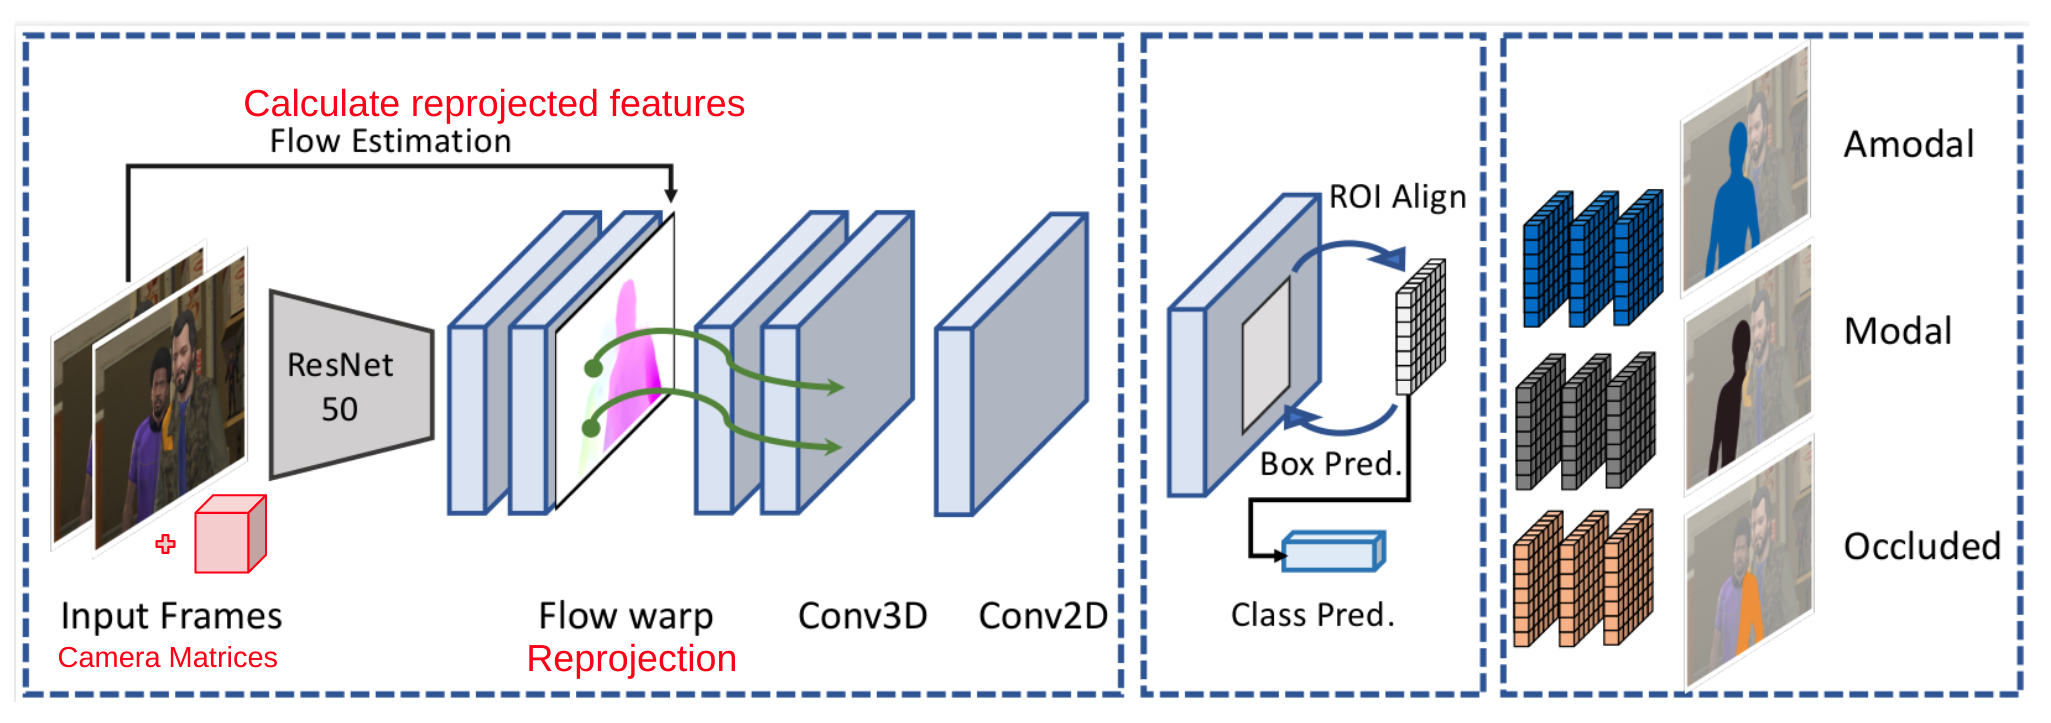
\includegraphics[width=0.97\textwidth]{fig/pipeline}
\vspace{-0.35cm}
\caption{Overview of our proposed framework for learning SAIL-VOS. Our Amodal-Net includes a temporal backbone, an iterative box-head and mask-head, while it is trained jointly with the task of modal and occlusion mask prediction.}
\vspace{-0.4cm}
\label{fig:pipeline}
\end{figure*}

Motivated by this capability, prior works~\cite{GuoECCV2012, SilbermanECCV2014b, KarICCV2015, LiECCV2016, zhu2017semantic, ehsani2018segan, follmann2019learning} studied the problem of amodal segmentation from a single image, \ie, the task of segmenting  both the visible \textit{and occluded} parts of an object.  
In meticulous work, Hu~\etal~\cite{hu2019sail} collected a dataset for  the task of Semantic Amodal Instance Level Video Object Segmentation (SAIL-VOS). Annotation of video data permits to expand amodal reasoning to the time dimension, which also seems crucial for human perception. However, the models proposed by Hu~\etal~\cite{hu2019sail} do not  take  advantage of the temporal information
and are mostly adapted from the modal instance segmentation task. 
While this is a very valuable first step, it is suboptimal for three reasons illustrated in. Specifically, missing temporal information prevents use of motion cues. Moreover, bounding boxes of amodal segmentations overlap much more significantly than those of modal masks. We found special treatment of this issue to improve results. In addition, amodal segmentation requires to deal with occlusions, \ie, object information from observations needs to be propagated more broadly.

To tackle these three challenges, Yeh and I proposed Amodal-Net, a framework for SAIL-VOS with a flow based temporal backbone, a redesigned box-head and a revised mask-head. 
More specifically, our temporal backbone enables the model to reason about occluded regions based on current and past frames. For this we incorporate temporal information into the amodal prediction model. Our box-head utilizes a cascade architecture with soft Non-Maximum Suppression (NMS) to address the challenge of heavily overlapping amodal boxes. Lastly, we developed a mask head with a large receptive field and self-attention to better propagate object information far into the occluded regions. 

Recently, Hu~\etal~\cite{HuCVPR2021} also collected detailed 3D information on SAIL-VOS. Intuitively, 3D information combined with temporal information will offer more clue for objects and their occlusion. Therefore, this thesis explores the effect of adding 3D information to the video data.  In particular, the model will incorporate depth map and camera intrinsic and extrinsic matrices into the input, and perform 3D reprojection in the feature space.


We evaluate our approach on the SAIL-VOS dataset~\cite{hu2019sail}, where we outperform state-of-the-art by $3.5\%$ (absolute-gain) in Average Precision (AP) on amodal video instance segmentation. 
We also investigate the effect of reprojection on the accuracy of our model on the SAIL-VOS dataset. Compared to the repreojection-less 
model, adding reprojection yields a minor improvemenet in AP, as well as a more significant improvement of $0.2$ when restricted to small 
objects.

%In order to extend our proposed methods into the standard amodal instance segmentation task and 
Next, to assess the generality of \textit{non-temporal} components in the base model,
%To the best of our knowledge, %~\cite{hu2019sail} 
%this is the only available video dataset. 
%To assess the generality of the \textit{non-temporal} components in \ourmodel, 
we also report results on the COCO-Amodal dataset~\cite{zhu2017semantic} and the KINS dataset~\cite{qi2019amodal}.
Our approach outperforms state-of-the-art by 4.0\% AP and 1.1\% AP respectively.
%\as{refer to fig.~1 and some nice illustrations where thingsg work.} 